\documentclass[sigconf]{acmart}

\usepackage{graphicx}
\usepackage{hyperref}
\usepackage{todonotes}

%\usepackage{endfloat}
%\renewcommand{\efloatseparator}{\mbox{}} % no new page between figures

\usepackage{booktabs} % For formal tables

\settopmatter{printacmref=false} % Removes citation information below abstract
\renewcommand\footnotetextcopyrightpermission[1]{} % removes footnote with conference information in first column
\pagestyle{plain} % removes running headers


\newcommand{\TODO}[1]{\todo[inline]{#1}}
\newcommand{\DONE}[1]{DONE: \todo[inline,color=green!30]{#1}}


\begin{document}
\title{Mapping the Social Network of Opioid Misuse on Twitter}


\author{Liz Supinski, Nandita Sathe, and Sean M. Shiverick}
\affiliation{%
  \institution{Indiana University-Bloomington}
  \institution{ILS-Z639: Social Media Mining - Spring 2018}
  \institution{Project Proposal: Group 1}
}
\email{smshiver@indiana.edu}

% The default list of authors is too long for headers}
\renewcommand{\shortauthors}{Supinski, Sathe, Shiverick}


%\begin{abstract}
%This paper provides a sample of a \LaTeX\ document which conforms,
%somewhat loosely, to the formatting guidelines for
%ACM SIG Proceedings.
%\end{abstract}

\keywords{Infodemiology, Prescription Opioids, Opioid Misuse, Social Networks, 
Twitter}

\maketitle


%%%%%%%%%%%%%%%%%%%%%%%%%%%%%%%%%%%%%%%%%%%%%%%%%%%%%%%%%%%%%%%%%%%%%%%%%%%%%%%%
\section{Introduction}

Over the past two decades, prescription opioid abuse and addiction in the U.S. 
has become a health crisis of epidemic proportion. Since 1999, the number of 
overdose deaths from prescription opioids, such as oxycodone and hydrocodone, 
has more than quadrupled \cite{nida18, cdc18}. Social media media mining (SMM) 
has been used to address public health concerns through “infodemiology” and 
“toxicovigilance”, which involves informatics for purposes of epidemiology, 
including strategies for monitoring patterns and prevalence of medication abuse 
\cite{eysenbach09, sarker16}. For example, researchers have tracked the outbreak 
of flu epidemics using internet searches and Twitter posts 
\cite{culotta10, paul14, lazer14}. Twitter data has also been used to track 
the expression of migraine headaches \cite{nascimento14}, detect misuse 
and abuse of prescription opioids \cite{sarker16, chary17, dzierak17}, and 
monitor illegal online sales of prescription opioids \cite{mackey17}. 
The relationship between Twitter posts and health outcomes is largely 
correlational, yet some research suggests that discussion of opioid misuse 
on Twitter may provide reinforcement for actual misuse of opioids 
\cite{hanson13}. Additional evidence would help to clarify the social network 
of Twitter users and the contexts of prescription opioid misuse. 

This project seeks to examine the relations among social media users posting 
content related to the misuse of prescription opioids (MUPO). Mapping social 
media content related to prescription opioid use may help detect individuals 
at risk for misusing prescription opioids, and identify factors related to 
opioid addiction. The main goal of this project is to map the social network
of prescription opioid misuse on Twitter. This proposal outlines several steps 
toward accomplishing this goal, which include: (a) Textual analysis of Twitter 
posts related to prescription opioid misuse, (b) Visualization of the 
geospatial location of Twitter users who post content on MUPO, and (c) Analysis 
of the social network of Twitter users who tweet about the MUPO. 

\subsection{Research Questions} 
\begin{enumerate}
    \item Can prescription opioid misuse be detected by Twitter posts? 
    \item Can we map the geographic location of  Twitter users discussing 
    prescription opioid misuse? 
    \item Can the social network of [prescription] opioid misuse be mapped 
    from Twitter users?  
\end{enumerate}

%%%%%%%%%%%%%%%%%%%%%%%%%%%%%%%%%%%%%%%%%%%%%%%%%%%%%%%%%%%%%%%%%%%%%%%%%%%%%%%%
\section{Literature Review} 

The misuse and abuse of opioids in the U.S. is a crisis with serious public 
health consequences. In 2015, an estimated 2 million Americans suffered from 
substance use disorders related to prescription opioid pain relievers 
\cite{nida18, cdc18}. Of patients legitimately prescribed opioids for chronic 
pain, between 21 to 29 percent misused them, 8 to 12 percent developed an 
opioid use disorder, and approximately 4 to 6 percent transitioned to heroin 
\cite{vowles15, carlson16}. Mobile health applications that monitor medication 
consumption have been developed to detect potential medication abuse 
\cite{varshney13}.

Infodemiology, broadly, the analysis of internet-sourced health data for public 
health research, is still in its infancy. One of the best known infodemiological 
successes is the forecast of flu outbreaks by analyzing the correlation between 
the frequency of flu-related Twitter posts and official reports of influenza-
like-illness from the CDC \cite{culotta10, paul14}. This research suggests that 
Twitter data can supplement official reports by providing information about the 
spread of flu 1 to 2 weeks earlier than the CDC-ILI. Because pharmaceutical 
manufacturers are obliged to monitor the safety of their drugs both before and 
after their release into the market, a field known as pharmacovigilance, the 
tools of infodemiology were quickly taken up in this field. Sarker and 
colleagues (2016) provide a methodological review studies using social media 
for pharmacovigilance, in which they point out that most studies rely on 
supervised learning with expert medical annotation of social media data 
\cite{sarker16}. 

In the area of prescription opioid misuse (MUPO), several works stand out. 
Chary and colleagues estimated misuse of prescription opioids from tweets, 
successfully detecting the incidence of tweets indicating opioid misuse with 
geographic incidence of opioid misuse as documented by the National Survey 
on Drug Use and Health (NSDUH) \cite{chary17}. This study used a customized 
version of Jiang-Conrath similarity algorithm \cite{jiang97} to determine the 
``kernal-weighted semantic distance'' between tweets and then used k-means 
clustering to separate tweets in opioid-misuse and non-opioid misuse 
categories. In a different study, Sarker et al. came up with a supervised 
classification technique to distinguish posts suggesting MUPO from non-MUPO 
posts \cite{sarker15}. Sarker and Gonzalez (2017) extended this work to present 
corpi for mining drug-related knowledge from Twitter using the `word2vec` tool 
to train shallow neural networks with two layers \cite{sarker17} They have 
continued to enhance these models since publication, and made their trained 
models available to researchers online 
(\url{https://data.mendeley.com/datasets/dwr4xn8kcv/3}). 
These models can be used for natural language processing using the `gensim` 
python library.

%%%%%%%%%%%%%%%%%%%%%%%%%%%%%%%%%%%%%%%%%%%%%%%%%%%%%%%%%%%%%%%%%%%%%%%%%%%%%%%%

Correlating twitter behavior with public health data requires that the twitter 
data be tied to geographic locations. Twitter geolocation is disabled by 
default and only a small number of users choose to enable it. It is estimated 
that only about 2 percent of tweets include geographic metadata, with the 
same prevalence found for GPS-tagged data \cite{chary17, leetaru13}. 
Chary and colleagues used a software program called `Carmen` to geolocate 
tweets without geodata. Carmen is a library for geolocating tweets, available 
in both Java and Python implementations which, given a tweet, will return 
Location objects that represent a physical location \cite{dredze13}. Carmen 
infers structured location information (country, state, county, city) using 
geocoordinates (if available) and and user profile information, but not tweet 
content. In an early paper on use of Twitter to explore health-related topics, 
Prier et al. (2011) used the Twitter search API parameter to retrieve tweets 
on a state-by-state basis \cite{prier11}. Twitter geosearch method is 
proprietary, but the Twitter search API documentation suggests a combination 
of device/gps coordinates, user provided profile location, and network/ip 
address are probably used to location to determine tweets that fit within 
the geocode search parameter \cite{twitterGet}.

%%%%%%%%%%%%%%%%%%%%%%%%%%%%%%%%%%%%%%%%%%%%%%%%%%%%%%%%%%%%%%%%%%%%%%%%%%%%%%%%

Like other behaviors, opioid misuse may spread by social contact. Spreading 
or diffusion of contagious disease occurs within contact networks of direct 
person-to-person interaction or other indirect pathways \cite{pastor01}. In 
the case of opioids, rather than describing persons as infected or uninfected, 
people may be considered as more or less susceptible to misuse, dependence, and 
addiction, depending on individual and environmental factors \cite{volkow14}. 
Furthermore, the structure of the contact network can influence epidemic 
spreading \cite{watts98}, as the \emph{small-world} property of many networks 
reveals that the distance between nodes is reduced by the pattern of 
connections within the network. In a social network any two random acquaintances 
may be connected, on average, by five to six intermediaries \cite{travers69}. 
Contact networks of drug use may have small-world properties as a few highly 
connected nodes can rapidly transmit contagion (i.e., drugs) throughout the 
network \cite{shaham03}. For simple contagion, weak ties among acquaintances or 
infrequent associations can also provide shortcuts between distant nodes within 
the network \cite{granovetter73}, and facilitate the spread of contagion or 
drug use. Social media research suggests that discussion of prescription drug 
abuse on Twitter is potentially reinforcing of medication abuse within an 
online social network \cite{hanson13}. Experimental evidence has also shown 
the structure of an artificially constructed online community influenced the 
spreading of behavior, as individuals who received reinforcement from multiple 
connections within their social network were more likely to adopt a behavior 
\cite{centola10}. Behavior also spread farther and faster through with 
small-world networks that are clustered and latticed than random networks.

%%%%%%%%%%%%%%%%%%%%%%%%%%%%%%%%%%%%%%%%%%%%%%%%%%%%%%%%%%%%%%%%%%%%%%%%%%%%%%%%

\subsection{Gap in the Literature} 

The literature reviewed above shows that previous research has analyzed the 
textual content of Twitter posts related to MUPO, the geographical location of 
Twitter users posting about MUPO, yet few studies have analyzed the structure 
of the social network of Twitter users discussing MUPO. The present study will 
partly replicate previous findings and address this gap in the literature by 
integrating different approaches to investigating MUPO in social media. Our 
proposal includes text analysis, geospatial mapping and network analysis to 
gain a better understanding of the structure of relations among Twitter users, 
to identify measures of centrality and community structure. 

\section{Data Description} 

Twitter provides a massive amount of information about individuals 
broadcasting their opinions, moods, and activities \cite{widener14}. This 
information is spatial as well as temporal. This project will analyze tweets 
between year 2015 to 2016 based on the following keywords below. We will use 
the Twitter API to extract the dataset. Our keyword list is derived from 
opioid-detection keywords in past research \cite{chary17, mackey17, lord11}, 
and ten most common prescription opioids from NSDUH-2015 \cite{shiverick17}
(NSDUH data for 2017 was not available, so we used recent data from 2015). 
The target terms for our investigation are: 
`oxycodone`, `oxycontin`, `hydrocodone`, `vicodin`, `codeine`, `percodan`, 
`percocet`, `lortab`, `lorcet`, `morphine`, `oxymorphone`, `hydromorphone`, 
`demerol`, `dilaudid`, `fentanyl`, `methadone`, `lomotil`, `kadian`, `avinza`, 
`duragesic`, `tramadol`, `buprenorphine`, `propoxyphene`, `roxanol`.

We will use a methodology similar to that described by Sarker and Gonzalez 
(2017), to enhance the list by including common street names and misspellings, 
aiming for a final keyword list of between 15-20 terms \cite{sarker17}. We 
will also extract latitude and longitude information of users from Twitter 
metadata \cite{twittergeo}. The spatial information will be used to map the 
geographic locations of Twitter users posting content about prescription
opioid misuse. We will also extract data to construct the network structure 
of relations among Twitter users. 

%%%%%%%%%%%%%%%%%%%%%%%%%%%%%%%%%%%%%%%%%%%%%%%%%%%%%%%%%%%%%%%%%%%%%%%%%%%%%%%%

\section{Research Design and Methods}
The main goals of the project are (i) to conduct textual analysis of Twitter 
posts based on MUPO keywords toprovide data for (ii) visualizing the geospatial 
location of Twitter users, and (iii) analyzing the social network of opioid 
misuse.  

\subsection{Textual analysis} 
We will preprocess data using the `IDIG` python module to detect language of 
tweets and discard non-English tweets. Standard lemmatization, stopword removal 
and conversion to lowercase will be done using the NLTK module. We will use 
a package for calculating semantic similarity to cluster Tweets \cite{chary17}, 
and may use a trained model in GENSIM to validate those clusters \cite{sarker17}. 
We will attempt to use k-means clustering to reduce these to two clusters, 
MUPO and non-MUPO tweets, for further analysis. If we need to resort to a 
supervised learning model to separate MUPO and non-MUPO tweets, we will 
consider using Mechanical Turk to collect classifications, as we do not have 
access to expert raters, and are curious to see if “layman” judgments are 
sufficient to build a model which correlates with public health data. 

%%%%%%%%%%%%%%%%%%%%%%%%%%%%%%%%%%%%%%%%%%%%%%%%%%%%%%%%%%%%%%%%%%%%%%%%%%%%%%%%
\subsection{Geospatial Visualization}

The project will identify and show the locations where Twitter users have 
posted about opioid misuse on a map \cite{twittergeo}. We will use Python 
module Carmen and/or Twitter search API geo-quering to increase the number of 
tweets with geographic information \cite{dredze13}. In addition to using this 
data for correlation analysis, we anticipate using the `plotly` python library 
to create an interactive map of MUPO data. Our project will use geotagged tweet 
location from the following sources: (a) Tweet Location: Twitter provides the 
option to geo-tag a Tweet as it is posted, (b) Mentioned Location: mention of 
locations in the Tweet content requires parsing the Tweet message for location 
names, including nicknames, and (c) Profile Location: Twitter Profile has a 
\emph{location} setting that can be filled out by the account owner; however, 
this information is not always provided \cite{widener14}. 

%%%%%%%%%%%%%%%%%%%%%%%%%%%%%%%%%%%%%%%%%%%%%%%%%%%%%%%%%%%%%%%%%%%%%%%%%%%%%%%%
\subsection{Network Analysis} 

The third part of the project involves extracting the network of connections 
between Twitter users posting about opioid misuse. This network is expected to 
be a directed, weighted graph, with several connected components. It may be 
appropriate to examine the network flow, determine the flow quantity, and 
measure the flow to each edge using a maximum flow algorithm such as the Ford-
Fulkerson algorithm \cite{zafarani14}. In addition, the Bridge detection 
algorithm can be used to identify underlying structure in the network by 
systematically removing key nodes or edges that connect components within the 
network. Other network characteristics of interest are density, connectedness, 
centrality, and community structure \cite{golbeck13}. Nodes with high 
betweenness centrality connect different clusters, and their removal can
isolate separate components or communities. In a comparison of supervised 
learning models, treatment, heroin use, cocaine use, and tranquilizer were 
identified as important features for classifying opioid misuse and abuse 
\cite{shiverick17}. It is hypothesized that the social network of Twitter 
users discussing opioid misuse may consist of separate components based on 
different aspects of opioid use. For example, some Twitter users may discuss 
prescribed medications versus synthetic or illicit opioids, whereas other 
Twitter users may post content related to treatment and recovery from opioid 
addiction. Detecting key nodes and edges that connect different components 
can identify different clusters or communities of opioid misuse on Twitter.

\begin{figure}[!ht]
  \centering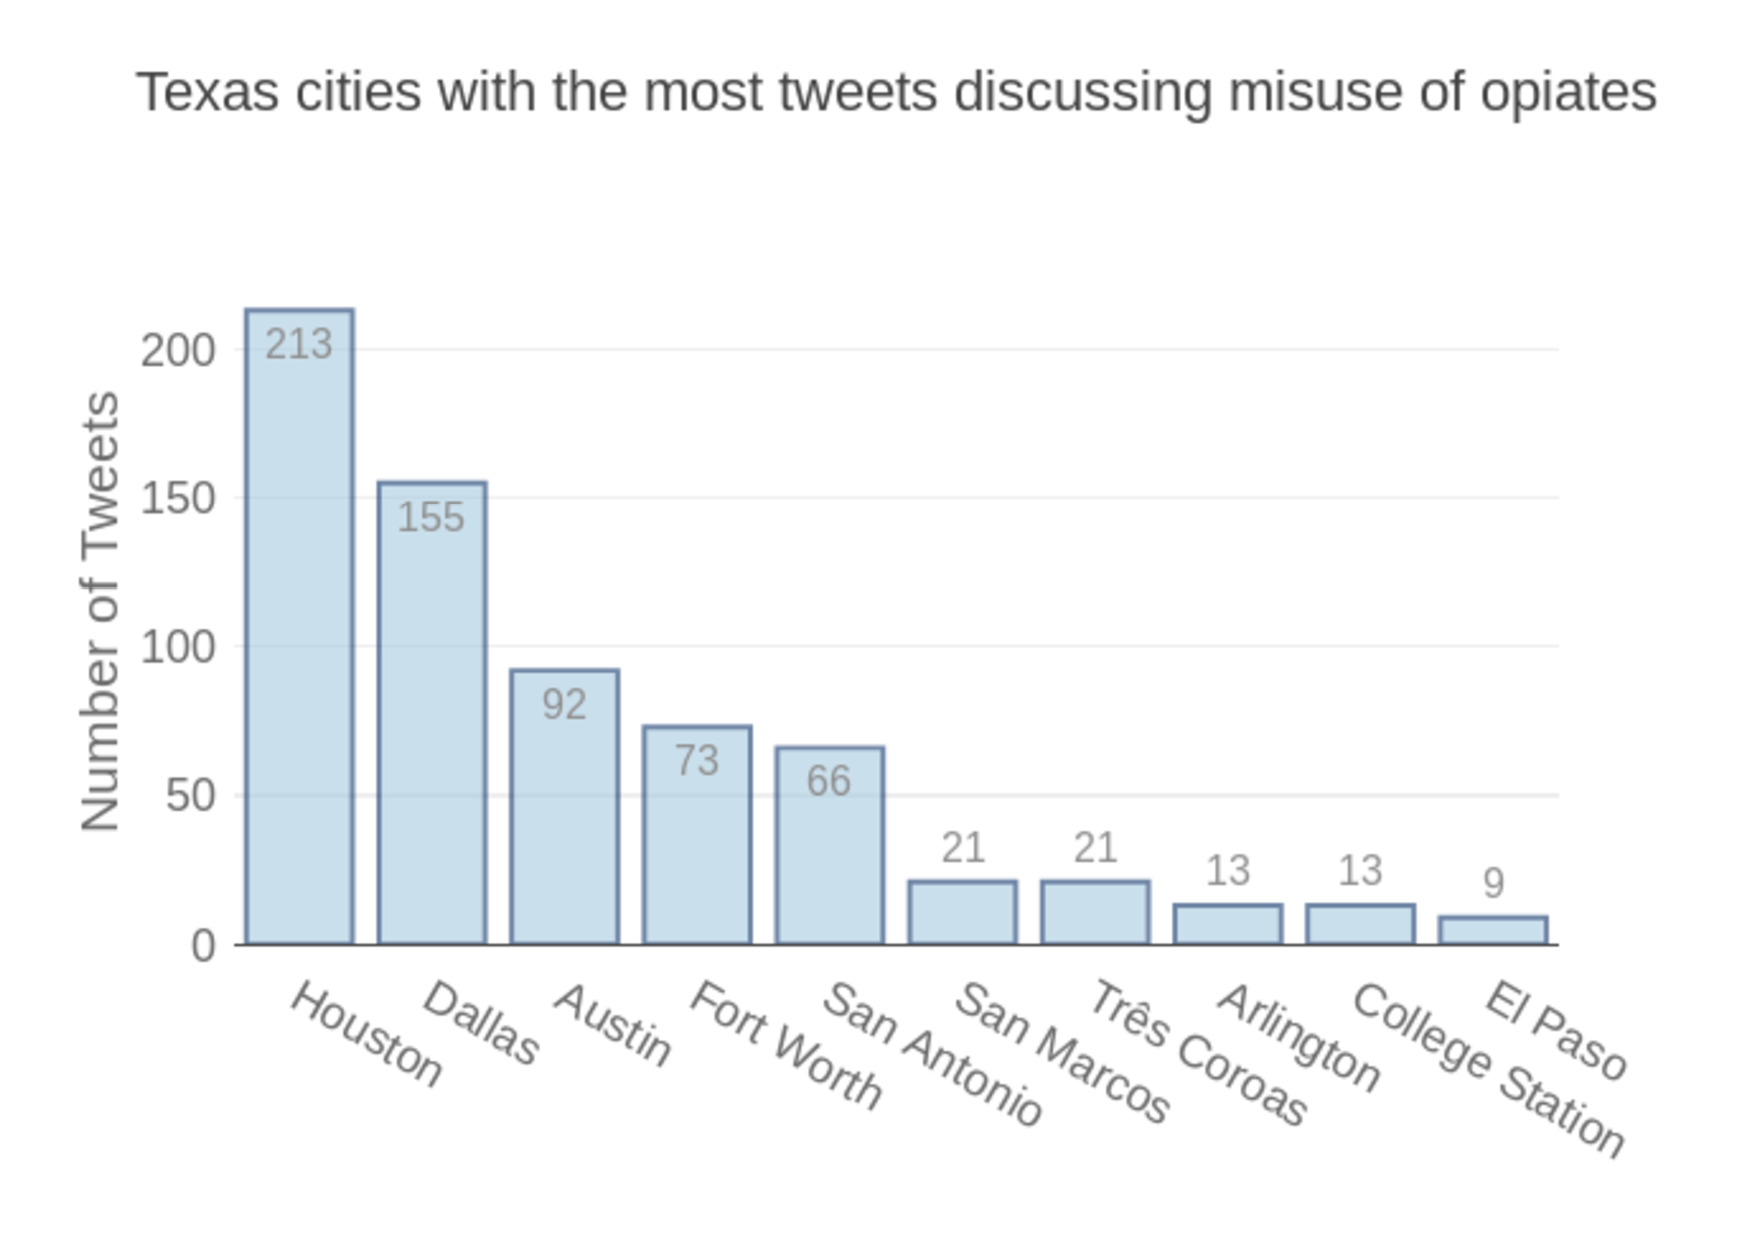
\includegraphics[width=\columnwidth]{images/Figure1.pdf}
  \caption{Network of Twitter Users Associated with Opioid Hashtag - 
  Observatory on Social Media IUNI}
  \label{f:Figure1}
\end{figure}

%%%%%%%%%%%%%%%%%%%%%%%%%%%%%%%%%%%%%%%%%%%%%%%%%%%%%%%%%%%%%%%%%%%%%%%%%%%%%%%%
\section{Conclusion}

To date, only a small amount of work using the tools of infodemiology to 
explore misuse of prescription opioids has been published. We aim to integrate 
several of the existing approaches to carry out correlational analysis with 
public health data that differs from others by foregoing the use of expert 
judges to support classification, and to extend our exploration into study to 
explore the structure of MUPO social networks, a nearly-unexplored direction 
to date. 

We believe that integrating methods of existing research and using 
updated data will provide additional support for the validity of twitter 
monitoring for MUPO. If our project approach is successful, it could provide 
the basis for the development of early warning systems for new MUPO hotspots, 
methods for university health officials to monitor changes in MUPO population 
behaviors or even tools for clinical monitoring of non-cancer chronic pain 
patients and other high-risk individuals. 
 
%%%%%%%%%%%%%%%%%%%%%%%%%%%%%%%%%%%%%%%%%%%%%%%%%%%%%%%%%%%%%%%%%%%%%%%%%%%%%%%%

%\begin{figure}[!ht]
%  \centering\includegraphics[width=\columnwidth]{images/fly.pdf}
%  \caption{Example caption}\label{f:fly}
%\end{figure}

% or generate them by hand while using the provided template in Table\ref{t:mytable}. 
% Note that the caption is before the tabular environment.

%\begin{table}[htb]
%\centering
%\caption{My caption}
%\label{t:mytabble}
%\begin{tabular}{lll}
%1 & 2 & 3 \\
%\hline
%4 & 5 & 6 \\
%7 & 8 & 9
%\end{tabular}
%\end{table}

%\begin{acks}
%  The authors would like to thank Dr. Gregor von Laszewski for his
%  support and suggestions to write this paper.
%\end{acks}

\bibliographystyle{unsrt}
\bibliography{report} 

%\appendix
%\input{issues}

\end{document}
